%	----- PACKAGES AND OPTIONS ----- 
\documentclass[11pt,a4paper,english,oneside]{article}
\usepackage{etex} %Because of many packages --> Extended TeX.
\usepackage[left=1in, right=1in]{geometry} %Helps to structure the paper layout.
\usepackage[Lenny]{./style/fncychap} %Design of the thesis.
\usepackage[utf8]{inputenc} %Due to vowels.
\usepackage[british]{babel} %Define the language style.
\usepackage{dsfont} %Nice style for the indicator function.
\usepackage{fancyhdr} %To customize the headers and footers.
\usepackage{booktabs} %In case you need \cmidrule or \addlinespace in tables.
\usepackage[hang,bottom,stable,multiple]{footmisc} %Style of footnotes.
%\usepackage{appendix} %For the \appendixpage command.
\usepackage[titletoc,toc,page]{appendix}
%Load some mathematical packages.
\usepackage{amsmath}
\usepackage{amsfonts}
\usepackage{amsmath}
\usepackage{amssymb}
\usepackage{mathtools}
\usepackage[sort,round]{natbib} %For the bibliography.
\usepackage{etoolbox} %To remove the page number on \appendixpage.
\usepackage{amsthm} %For theorems, definitions etc.
\usepackage{thmtools} %For theorems, definitions etc.
\usepackage{setspace} %Use double spacing.
\usepackage{lipsum} %For the \lipsum command to generate a text.
\usepackage{datetime} %For the specification of the date.
%\usepackage{tocloft} %The ToC, LoF and LoT each appear not necessarily on a new page.
\usepackage{graphicx,listings,xcolor,textcomp} %For the graphics, listings etc.
% \usepackage[justification=raggedright,singlelinecheck=true,
%              font=small, labelfont=bf]{caption} %Customize the captions.
\usepackage{caption,threeparttable}
\captionsetup{labelfont=bf,
              justification=raggedright,
              singlelinecheck=false,
              labelfont=bf,
              font=small}
% \usepackage[justification=raggedright,
%             singlelinecheck=false,format=plain]{subcaption}
\usepackage{chngcntr} %To use counterwithout.
\usepackage{epstopdf} %For inserting .eps files into the document.
\usepackage{xparse} %Load for \NewDocumentCommand command.
\usepackage{rotating} %To rotate a table.
\usepackage{pdfpages}
\usepackage{array,hhline} %To create tables and matrices.
\usepackage{tabularx} %An extended version of tabular.
% \usepackage{arydshln} %Due to the capability to draw horizontal/vertical dash-lines.
\usepackage{hyperref} %Must be loaded at the end.
\usepackage{cleveref} %For the command \cref, load after hyperref.
\usepackage{makecell}
\usepackage{cellspace}
\setlength\cellspacetoplimit{4pt}
\setlength\cellspacebottomlimit{4pt}

\graphicspath{ {./../resources/figures/} } %  Figures directory

\renewcommand{\appendixpagename}{\appendixname}
\renewcommand{\appendixtocname}{\appendixname}

\noappendicestocpagenum

%Setup of the reference links.
\hypersetup{
     colorlinks=false,
     linkcolor=blue,
     citecolor=blue,
     filecolor=magenta,
     urlcolor=blue}

%Define some reasonable margins.
\setlength{\textwidth}{6.6in}
\setlength{\textheight}{8.8in}
\setlength{\topmargin}{-0.1in}
\setlength{\oddsidemargin}{0in}
\setlength{\parskip}{1mm}

\bibliographystyle{abbrvnat} %Reference style.
\allowdisplaybreaks[1] %Page breaks of equations are allowed, but avoided if possible. 2-4 more relaxed.

%New command for the UZH logo.
\newcommand*{\plogo}{
\includegraphics{./style/uzh_logo_e_pos}}

%New command for the differential d to have an ordinary d.
\makeatletter
  \newcommand{\ud}{\mathrm{d}}
\makeatother

%Remove page number on \appendixpage. Use the package 'etoolbox'.
\makeatletter
\patchcmd{\@chap@pppage}{\thispagestyle{plain}}{\thispagestyle{empty}}{}{}
\makeatother

%Declare Definitions, Theorems etc.

%Readjust the numbering.
%\counterwithout{footnote}{chapter}
%\numberwithin{equation}{chapter}

\setlength{\parindent}{0cm} % Uncomment this if you don't want to have indents.

%	----- TITLE PAGE ----- 
\newcommand*{\titleGP}{\begingroup %Create the command for including the title page in the document.
\centering %Center all text.
\vspace*{\baselineskip} %White space at the top of the page.
\plogo\\[2\baselineskip] %University Logo.
\rule{\textwidth}{1.6pt}\vspace*{-\baselineskip}\vspace*{2pt} %Thick horizontal line.
\rule{\textwidth}{0.4pt}\\[\baselineskip] %Thin horizontal line.
{\LARGE Scarcity channel of Quantitative Easing :}

\vspace*{3pt}

{\LARGE Examining the Overnight Treasury Repo Market in the US}\\[0.2\baselineskip] %Title.
\rule{\textwidth}{0.4pt}\vspace*{-\baselineskip}\vspace{3.2pt} %Thin horizontal line.
\rule{\textwidth}{1.6pt}\\[2\baselineskip] %Thick horizontal line.
\scshape %Small caps.
Master's Thesis\\[2\baselineskip]
Submitted in partial fulfillment of the requirements for the degree of Master of Arts in Economics and Business Administration \par
\vspace*{2\baselineskip}
Author\\
{\Large Hubert Mrugala \\ [5pt]
 }
Seemattweg 4, 6315 Oberageri \\[5pt]
19-764-265 \\[5pt]
hubert.mrugala@uzh.ch \\


\vspace*{2\baselineskip}
Supervisor\\
{\Large Prof. Dr. Kjell Nyborg\\[5pt]\small Chaired Professor of Finance\\[5pt]
\small Department of Banking and Finance\\[5pt]University of Zurich\par}
\vspace*{2\baselineskip}
Assistant\\
{\Large Benjamin Schneider \par}
\vfill
{\scshape Date of Submission: \textcolor{red}{DRAFT}} \\[0.3\baselineskip] % 18.05.2022
\endgroup}

% ----- SPECIAL HEADER AND FOOTER STYLE  ----- 
% for the executive summary and Task Assignment section.
\fancypagestyle{firststyle}{%
  \fancyhf{}%
  \renewcommand{\headrulewidth}{0pt}
  \fancyfoot[C]{\thepage}}

%Customize headers and footers.
\pagestyle{fancy}
\fancyhead[R]{\thepage}
\fancyhead[L]{\rightmark}
\fancyfoot[L]{Hubert Mrugala}
\fancyfoot[C]{}
\fancyfoot[R]{Scarcity channel of Quantitative Easing}

%Define the signature line with dots.
\NewDocumentCommand \dotbox {o O{.5\linewidth} m O{3ex} O{\linewidth}}
{
  \begin{minipage}{7cm}
    \makebox[7cm][l]{\,.\dotfill}
    \\
    \makebox[7cm][l]{\,#3}
  \end{minipage}
}

% ----- BEGIN DOC AND PROJECT DEFINITION ----- 
\begin{document}

\thispagestyle{empty}
\titleGP
\newpage
\doublespacing
\setcounter{page}{1}
\pagenumbering{Roman}
\section*{Task Assignment}

\begin{figure}[h!]
  \begin{center}
    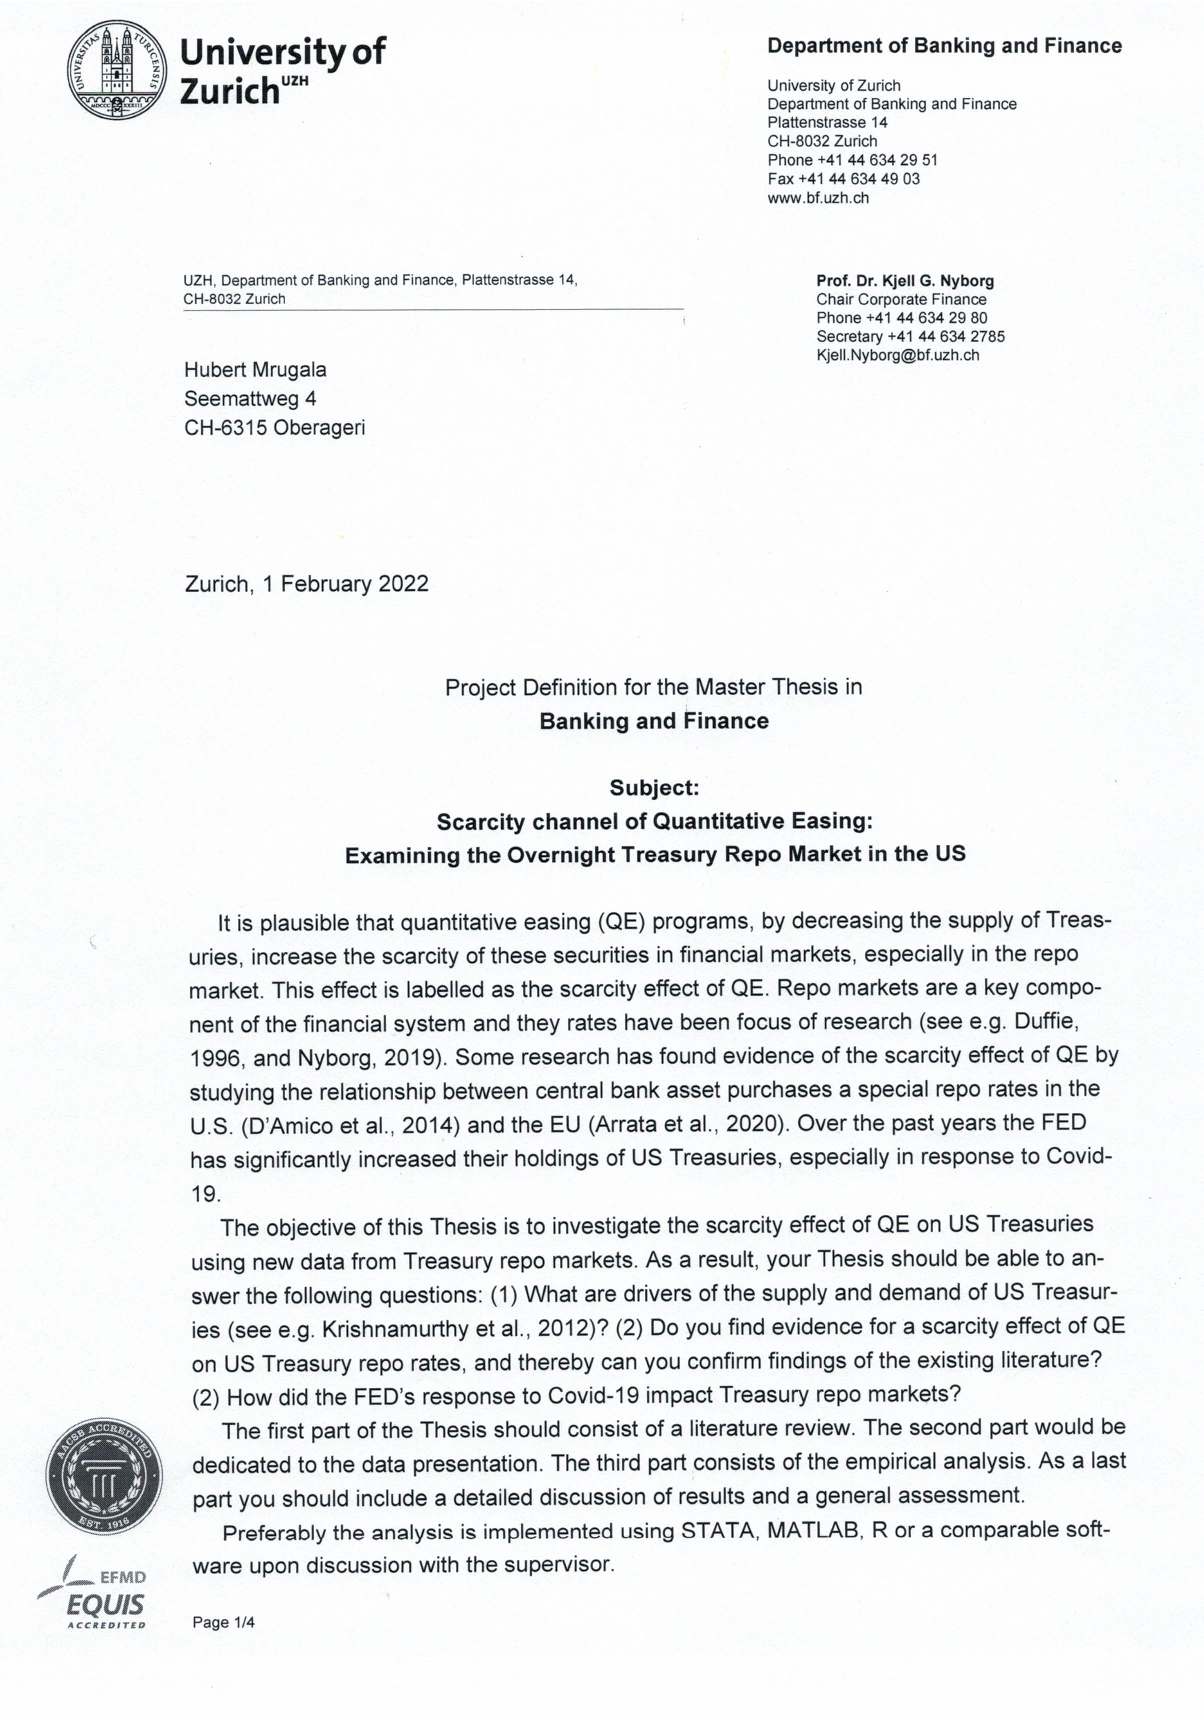
\includegraphics[page=1,width=.86\textwidth]{../../project_definition.pdf}
  \end{center}
\end{figure}
\newpage
\begin{figure}[h!]
  \begin{center}
    \includegraphics[page=2,width=.86\textwidth]{../../project_definition.pdf}
  \end{center}
\end{figure}
\newpage
\begin{figure}[h!]
  \begin{center}
    \includegraphics[page=3,width=.86\textwidth]{../../project_definition.pdf}
  \end{center}
\end{figure}
\newpage
\begin{figure}[h!]
  \begin{center}
    \includegraphics[page=4,width=.86\textwidth]{../../project_definition.pdf}
  \end{center}
\end{figure}

\thispagestyle{firststyle}
\newpage

% ----- EXEC SUMMARY AND ABSTRACT ----- 
\section*{Executive Summary}
\thispagestyle{firststyle}

\lipsum[1-3] % Here goes the text

\newpage
\tableofcontents
\newpage
\listoffigures
\newpage
\listoftables
\newpage
\pagenumbering{arabic}

\begin{center}
  {\Large \emph{\textbf{Scarcity channel of Quantitative Easing:\\
  Examining the Overnight Treasury Repo Market in the US}}}\\[4pt]
  Hubert Mrugala
\end{center}

\abstract{\lipsum[1]}

\begin{flushleft}
  \textbf{JEL classification}: E4, E5\\
  \textbf{Keyword}: Collateral, Scarcity, Treasury, Monetary Policy, Repo Market
\end{flushleft}

% ----- INTRODUCTION ----- 
\section{Introduction} \label{sec:introduction} % 3.5 - 4 pages

The COVID-19 pandemic has caused the deepest US recession since the Great Depression and induced the biggest monetary stimulus since the Global Financial Crisis. One of the monetary policy tools that was activated during the pandemic was an additional round of quantitative easing.\footnote{It was actually an acceleration of already present QE that was sparked by 2019 repo rumble.} In the time of 4 months, the Fed's balance sheet exploded from \$4.2 to \$7.1 trillion, and then kept growing. As of April 2022, total assets of the Fed reached almost \$9 trillion. Central bank asset purchases are used in normal times as a unconventional policy that helps achieving ultimate goals of the Fed, which are maximum employment and inflation level at 2\% over the longer run.

There are many theoretical transmission channels of quantitative easing, however almost all of those channels focus on positive effects of asset purchases. Negatives are very rarely analysed. \citet{nyborg2015} showed that collateral frameworks of ECB distort financial markets' efficiency by making bad collateral look better then it really is. What about a high-quality collateral? Can draining fist-class collateral out of the markets have an adverse impact on the economy?

There is one channel of quantitative easing that is rarely mentioned and insuffitiently studied.\footnote{In financial media, only Izabella Kaminska of FT Alphaville sometimes covered collateral scarcity.}. It is the scarcity channel (or scarcity effects). While most channels on QE focus on abundance of reserves, central bank liquidity, the scarcity effect, puts emphasis on the collateral-side of the swap, which is the public sector liquidity. There are only two academic papers that study the scarcity channel of asset purchases programmes. \citet{damico2014} find that there was a scarcity premium of US Treasury securities traded in the repo market during the time of LSAP programs. Likewise, \citet{arrata2018} determine a similar relationship in the \textbf{Euro zone market for repo contracts}. Both papers prove the existence of the scarcity effects in the US and EU markets, however, those investigations look only at specific special repo markets and don't take into account the mechanics of the collateral intermediation complex. Furthermore, there hasn't been any research done about the scarcity premium of US Treasuries in over eight years, despite an almost constant QE during that period.

This research fills the subject gap, the time gap, and the context gap in the narrow literature on scarcity effects. I use a General Collateral Financing Treasury Repo rate weighted index in a timespan of the last 15 years to test a connection between the level of US Treasury securities on the Fed's balance sheet and the index. Additionally, to focus completely on the collateral-side of a repo transaction, I use a collateral spread as the dependent variable. \citet{nyborg2019b} \textbf{find ...}

\textbf{[Findings]}

I control for \textbf{[...]} and emphasize the importance of high-quality collateral by describing its dynamics and economic function. Moreover, I add an innovative proxy for the re-use rate of collateral in the banking system as an extension of the base model.

The research connects three different strains of literature, which are research on collateral scarcity, US Treasury markets and collateral intermediation.

Apart from already mentioned academic papers on scarcity effects, there is also one investigation of the Japanse JGB market that contributes to the literature on collateral scarcity. \citet{han2018} have documented that BoJ purchases of Japanese Government Bonds in QE and then QQE programs have negative impact on market liquidity, which suggest scarcity effects.

The second stain is the literature on repo market rates and cash market rates of US Treasuries. The work of \citet{duffie1996} introduced a model that shows how short-selling Treasuries obtained by reverse-repo transactions can create squeezes at delivery dates and so, cause some repos to trade on special. Special repo rates are not studied in this research, however, mechanics of special repos are important because US Treasuries, as a whole asset group, are special on their own. \citet{krishnamurthy2012} show that yields of US Treasury securities have a non-default component that makes them trade at a significant premiu. 

The last branch of literature is concerned with the collateral supply and its intermediation. \citet{singh2011} shows how collateral agency is embedded into the shadow banking system. \citet{sissoko2020} show how sufficient collateral supply is crucial to properly functioning money markets and effective monetary policy. \citet{singh2012} introduce and explain a phenomenon of "collateral-chains". \citet{singh2017} calculates the collateral re-use rate that represents endogenous shadow creation of collateral. \citet{jank2020} finds a positive relationship between ECB bond purchases (PSPP) and the re-use rate of collateral suggesting that the market participants adjust to shocks in collateral scarcity by utilizing more source collateral.

Investigating scarcity effects of unconventional monetary policy is important because it is not certain that government bond purchasing programs of central banks have a net positive effect on the real economy. Benefits of QE or PSPP are not clear. Despite over 10 years of bloated central bank balance sheets, inflation and growth did not follow.\footnote{According to \citet{gern2015}, increase in GDP and inflation are two final effects of the QE/PSPP transmission mechanism.}. If scarcity effects are large and significant, then a lack of central bank unsterilized actions in response to an external shock may be more beneficial than active bond purchases. Nonetheless, the final assessment must be made by looking at the bigger picture and taking into account other factors like the regulatory environment and demand for reserves. This work studies only scarcity effects. \textbf{Last but not least, scarcity effects and connection to .. may shed a light on why some central banks decide to apply controvenial collateral frameworks.}

\begin{figure}[htb!]
  \begin{center}
    \caption{The long-term rate has been very low in spite of massive QE}
    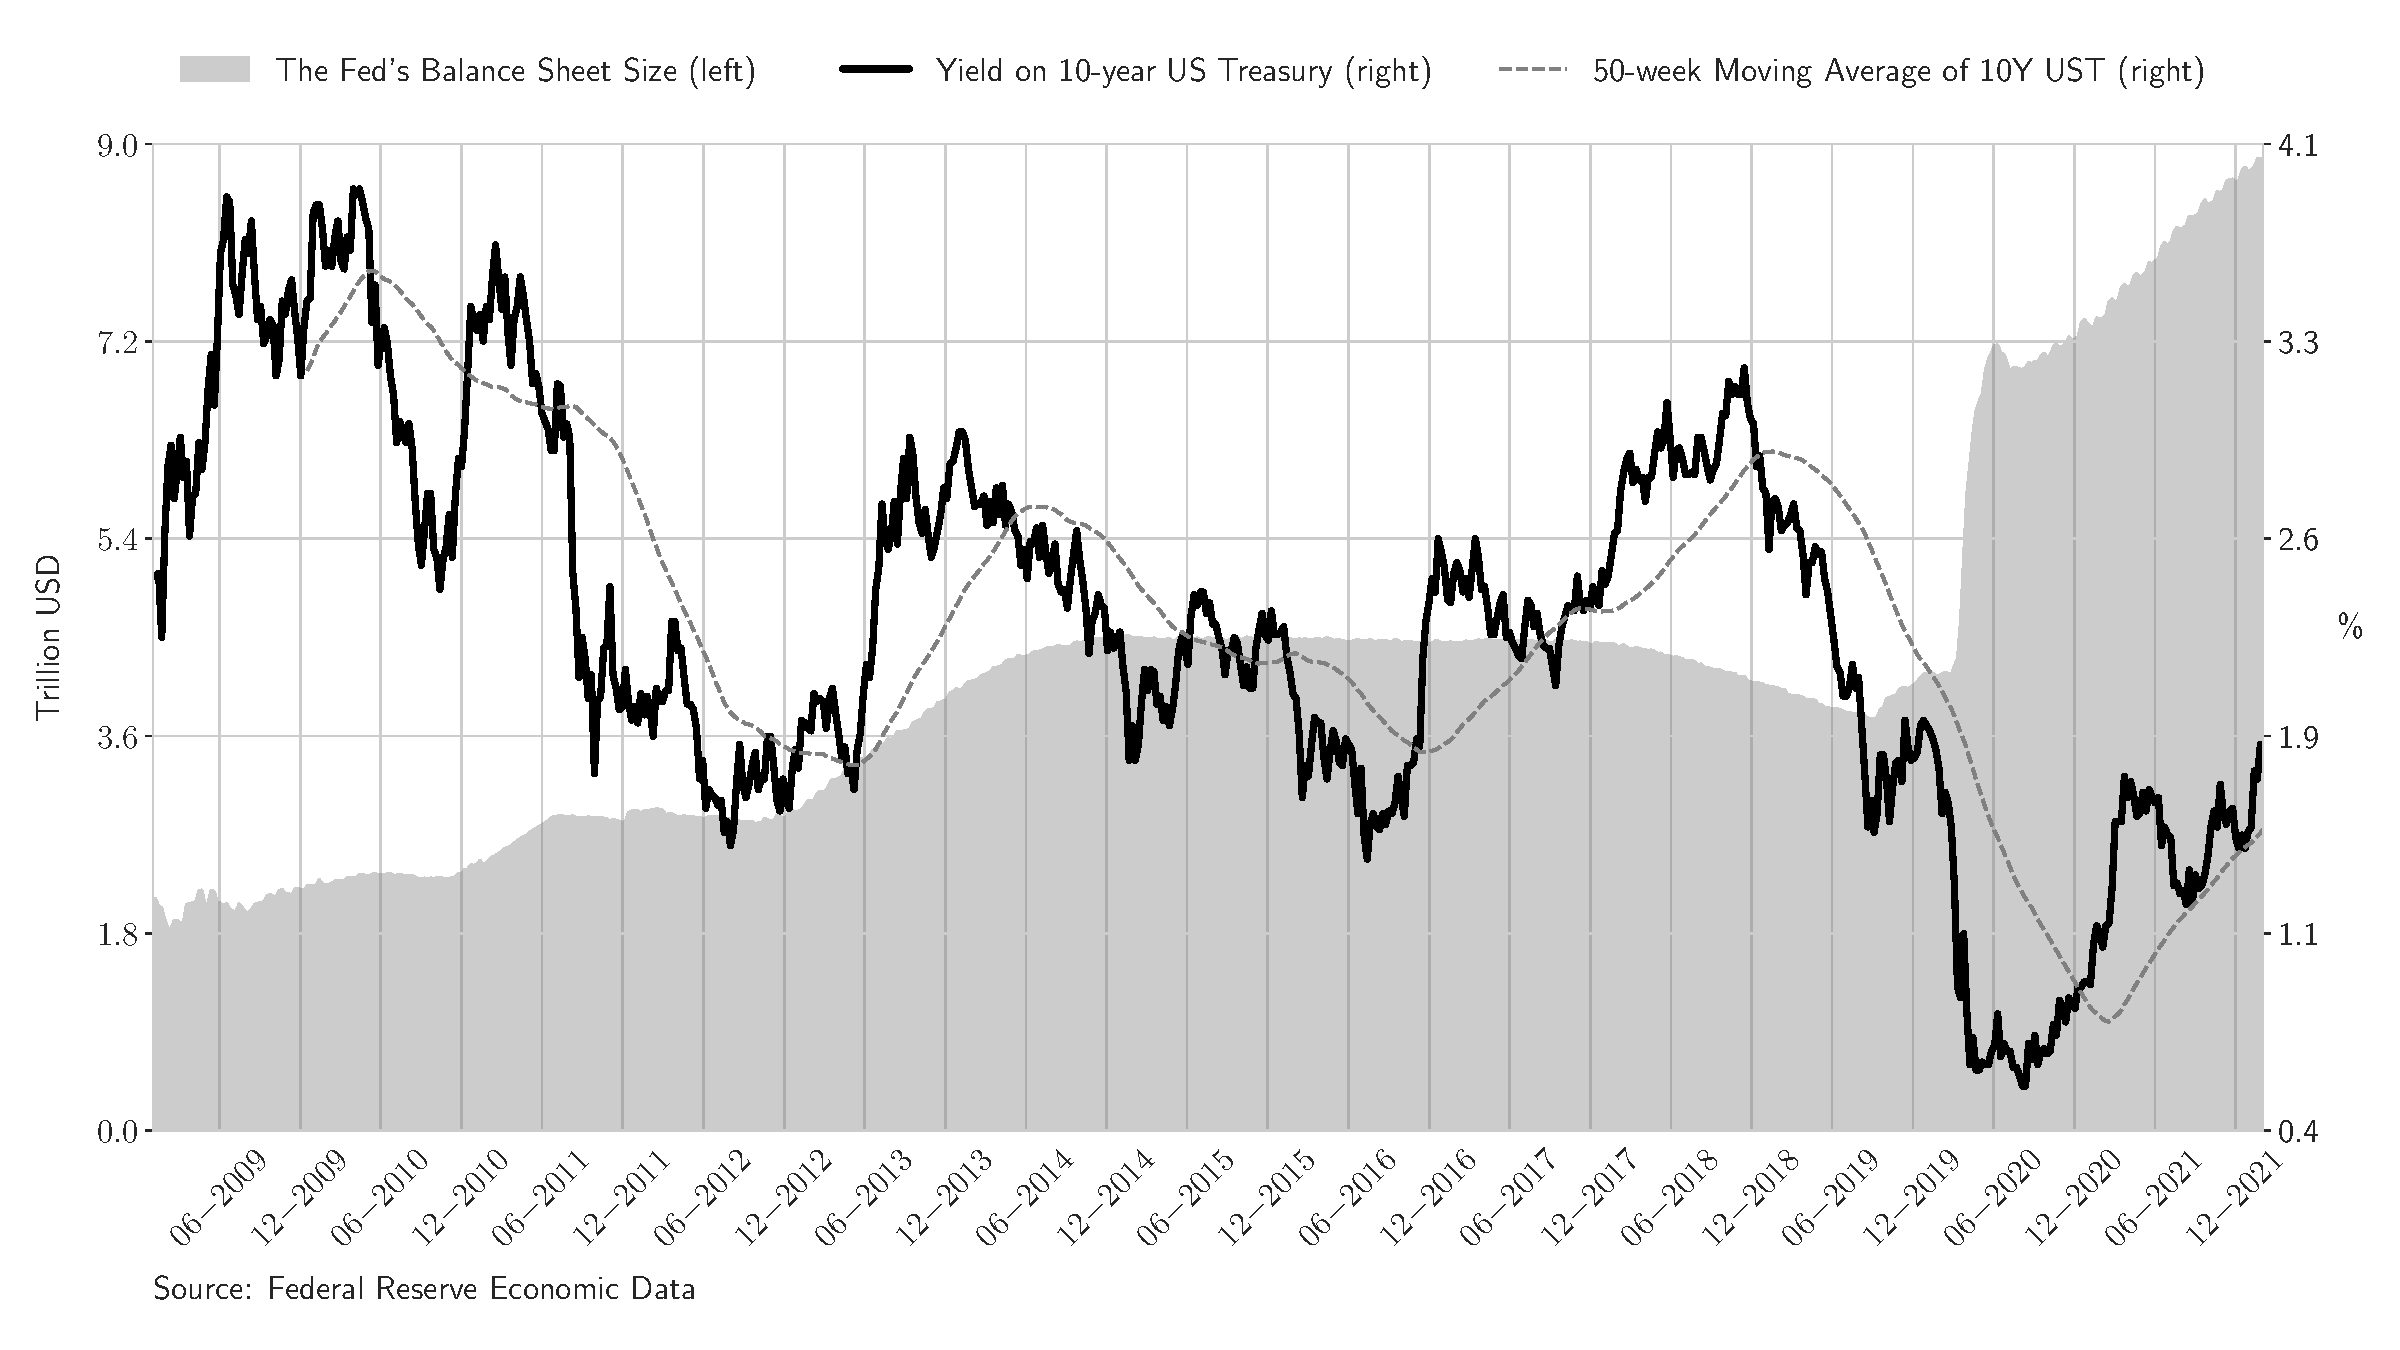
\includegraphics[width=0.99\linewidth]{fed_bs.pdf}
  \end{center}
  \label{Feds_BS}
\end{figure}

The remainder of the paper is organized as follows. \textbf{Section two. Section three.} The last section concludes.

\newpage

% ----- COLLATERAL MECHANICS ----- 
\section{Mechanics of collateral} \label{sec:mechanics} % 3-4 pages

\lipsum[1-20]

% ----- COLLATERAL SHORTAGE ----- 
\section{Collateral shortage in years 2020-2022} \label{sec:shortage}% 3-4 pages 

\lipsum[1-20]

% ----- EMPIRICAL ----- 
\section{Empirical tests} \label{sec:empirical}

\subsection{Data} % 2 pages

The main variables that are studied in this research are: Fed's SOMA Treasury holdings, GCF treasury Overnight repo rate and the USD collateral spread.

Repo rate data comes form The Depository Trust \& Clearing Corporation (DTCC). The rate is a weighted-average rate of repo contracts that are backed with repo-eligible Treasuries with maturity less than 30 years (CUSIP: 371487AE9). It tracks the average daily interest rate paid for the most-traded GCF Repo contracts for US Treasury securities. DTCC a of clearing house for trading US government securities.

Collateral spread is the difference between an unsecured and secured money market rate. Unsecured financing normally is more expensive that a secured one, since secured lending (e.g. a repo contract) is safer to the leg that lends legal tender money. That is not always the case as showed in figure \ref{fig:collateral spread}. \citet{nyborg2019a} explains what drives collateral spread and makes at times to turn negative. Here, the collateral spread, for the US market, is defined as the difference between overnight USD LIBOR rate and the overnight GCF Treasury repo rate. Expressing the repo rate in the form of a collateral spread is important when analysing dynamics of collateral and it's impact on money markets. % It is because a collateral spread expresses the premium lenders pay for security.

Scarcity effects should be most visible in the repo rate because engaging in a reverse repo contract is the cheapest way of obtaining collateral securities. This analysis uses a general collateral repo rate, as opposed to a special repo rate. The reason for such decision is twofold. First, there haven't been done any studies on scarcity effects that investigate a GC repo rate on a macro level. Second, data for the rate is easily accessible online. Using a GC rate is convinient because of the fact, that in regression studies, there is no need to control for specialness and short selling. On the other hand, it is hard to include the market microstructure factors when using a general collateral rate, especially with the weekly data frequency that is applied in this study.

To gauge the volume of Treasury securities on the Federal Reserve balance sheet, I use the System Open Market Account Holdings (SOMA) data. SOMA holding are Fed's assets acquired via open market operations. To make the data relevant for this study, I sum only Treasury bills, notes and bonds and leave out mortgage backed securities and federal agency securities.

Increase in the Fed's SOMA Treasury holdings reduce the supply of government security collateral, however, increase in the outstanding security debt has the opposite effect. I use Debt to Penny daily data of all federal debt outstanding, except debt held by intragovernmental holdings. This time-series is re-sampled to weekly Wednesday levels to match the frequency of the Fed's Treasury holdings.

The recently popular reverse repo standing facility of the Federal Reserve can alleviate any potential shortage of Treasury collateral, thus I also include these figures as well. For a more detailed analysis of the Fed's RRP sale volumes, please see section \ref{sec:shortage}.

To control for other factors that move the repo rate and collateral spread I include three other variables, namely VIX index, 1-month yield on US Treasury bill and a yield curve defined as 10-year UST yield less 3-month UST yield. All non-dummy variables are defined in table \ref{table:variables}.

Lastly, there are four categorical variables used to control for changes in the Fed's monetary policy stance. Two of them show when the Fed rises or lowers the fed funds target rates, and the other two indicate dates when the Fed expands and normalizes its balance sheet. The dates can be seen in table \ref{table:dates}, in the appendix section.

% Table: Variables
\begin{sidewaystable}[htbp!] \centering
\caption{Explanation of variables.\\
  All data was accessed and transformed on 10th March 2022.}
{\renewcommand{\arraystretch}{2.2} 
\begin{tabular}{lll}
\toprule
  \textbf{Variable} & \textbf{Definition} & \textbf{Source} \\
\midrule
  TREASURY REPO RATE &  \makecell[l]{GCF (General Collateral Finance) Treasury repo rate\\weighed index composed of GCF repo-eligible CUSIPs:\\U. S. Treasury $<$ 30-year maturity, in bps} & www.dtcc.com\\
\hline
  LIBOR & ICE "Panel Bank" Overnight USD LIBOR rate, in bps & Bloomberg\\
\hline
  COLLATERAL SPREAD & USD ON LIBOR rate minus the Treasury repo rate, in bps & \\
\hline
  UST 1M & Yield on generic 1-month US Treasury bill, in bps & home.treasury.gov\\
\hline
  YIELD CURVE & \makecell[l]{10-year US Treasury note yield  minus 3-month US Treasury\\bill yield, in bps} & home.treasury.gov\\
\hline
  SOMA TREASURIES & \makecell[l]{Fed's Treasury securities at System Open Market\\Account holdings, tril USD} & www.newyorkfed.org\\
\hline
  DEBT & Debt held by the public (debt to penny data), in tril USD & fiscaldata.treasury.gov\\
\hline
  RRP & \makecell[l]{Fed's Overnight Reverse Repurchase Agreements -- Treasury\\securities sold by the Federal Reserve in the temporary\\Open Market Operations, in tril USD} & fred.stlouisfed.org\\
\hline
  VIX & Chicago Board Options Exchange's CBOE Volatility Index & finance.yahoo.com\\
\hline
  PD FAILS & \makecell[l]{Repo fails to receive and fails to deliver, US Treasury\\securities, Primary Dealer Statistics, in tril USD} & www.newyorkfed.org \\
  \bottomrule
\end{tabular}}
% \begin{flushleft}
% \hspace{35pt}\textit{* .}
% \end{flushleft}
\label{table:variables}
\end{sidewaystable}

The time range of the whole data set\footnote{Except primary dealer statistics data that is used in one regression in the appendix.} goes from January 2, 2008 to December 29, 2021. All data has weekly frequency, Wednesday levels. Dollar values are in trillion USD, rate values are in basis points (bps). Table \ref{table:stats} shows descriptive statistics of the data used in regression analysis. All of the data, except the LIBOR rate, comes from free online resources. For detail, please see table \ref{table:variables}.

% Expand this section by adding details about those varaibles

\subsection{Descriptive Statistics}

\lipsum[1-3]

% describe shortly the data

% table + plot 3x horizontal repo rate, collateral spread, soma holdings

% describe shortly the data

% Table: Statistics
\begin{table}[!h] \centering
\begin{threeparttable}
\caption{Descriptive statistics.\\Observations from January 2, 2008 to January 5, 2022 (except the last variable which data starts from April 3, 2013). The data below is not transformed, however, regressions in the following section apply first-differencing.}
\begin{tabular}{lrrrrr}
\toprule
{} &    mean &    min &     max &    std &  obs \\
\midrule
  GCF Treasury ON repo rate (bps)      &   64.00 & -19.30 &  418.40 &  82.63 &  732 \\
Collateral spread, USD (bps) &    2.89 & -47.11 &  495.28 &  29.63 &  731 \\
ON USD LIBOR rate (bps)             &   66.97 &   5.46 &  509.38 &  87.47 &  731 \\
1-month UST yield (bps)           &    0.52 &   0.00 &    3.37 &   0.77 &  732 \\
10-year less 3-month UST yield (bps)       &  183.24 & -49.00 &  380.00 &  96.53 &  732 \\
  Treasury SOMA holdings (tril USD)     &    3.54 &   0.47 &    8.23 &   1.74 &  729 \\
  Treasury debt outstanding (tril USD)              &   13.00 &   5.10 &   23.03 &   4.47 &  732 \\
  Fed's RRP standing facility volume (tril USD)               &    0.09 &   0.00 &    1.70 &   0.25 &  732 \\
VIX volatility index              &   20.15 &   9.19 &   80.86 &   9.76 &  732 \\
  Treasury security repo fails (all fails)          &    0.19 &   0.06 &    0.89 &   0.11 &  457 \\
\bottomrule
\end{tabular}
\label{table:stats}
\end{threeparttable}
\end{table}

\subsection{Base regression specification} % 2 pages

The main objective of this paper is to determine whether Fed's Treasury buying programs make Treasury securities more scarce in the market. To see that, I test a casual connection between Treasury security supply factors and the GCF Treasury repo rate with a simple linear regression. All data put into regressions is in first differences in order to remove trends and make time-series stationary.

There are two sets of OLS regressions with two different dependent variables. My basic regression specification involves the general collateral repo rate as the dependent variable and a set of independent variables that reflect supply and demand factors for collateral. The following is the base regression equation

\begin{equation} \label{eq:1}
  \begin{gathered}
  \Delta \textit{Treasury Repo Rate} = \beta_0 + \beta_1 \Delta \textit{SOMA Treasury}_t + \beta_2 \Delta \textit{Debt}_t \\ + \beta_3 \Delta \textit{RRP}_t  + \beta_4 \Delta \textit{UST 1M}_t + \gamma \textit{Controls}_{i,t}
  \end{gathered}
\end{equation}

$\Delta$ SOMA Treasury and $\Delta$ Debt variables are supply factors of the underlying collateral. The former shows to what extend the Fed draws Treasury securities out of the market and the latter variables represents provision of collateral to the market.

Fed's RRP standing facility sales are initiated by agents that seek to lend reserves to the central bank. Therefore, Treasury sales that go through the RRP facility are a demand factor for collateral. RRP volume alone cannot capture all of the demand that exist for liquid Treasury securities. It is so because only eligible parties can access central bank facilities and the price of those reverse-repo contracts is set only by the Fed. In order to account for demand for Treasury securities in the wider market, I use the $\Delta$ UST 1M variable, which is a yield on generic one month Treasury bill. \textbf{The quality of the underlying collateral affects repo rates as showed by Bartolini et al and Nyborg. Consequently, as the yield of the underlying security rises, the repo rate should also increase}.

% Controls

To capture the effect of other determinants of the repo rate I incorporate three more macro variables, as well as four categorical variables that control for changes in monetary policy. Those additional macro variables are the VIX stock volatility index and the UST yield curve.

\subsection{Problem with the unsecured rate}

Repo contracts aren't all about the collateral but also serve as an instrument that provides cash liquidity to the buyer. Sometimes repo rates react more to the "collateral leg", that's when the rates plummet, but usually repo rates respond more to the "cash leg", that is driven by the demand for funds. Thus, it is essential to account for demand for cash liquidity factor, that is not associated with collateral when examining repo rates.

The unsecured rate, which in this case is the US dollar O/N LIBOR rate is an important component that indicates the price of dollar liquidity. However, it would be reckless to include it in the regression as a right-hand side variable because of a potential reverse causality problem.

Since the Global Financial Crisis, activity in the unsecured money market segment have been declining. In 2003, the split of the total lending turnover was roughly equal, but by 2015 the size of the unsecured market was only one-tenth of total \citet{fiore2018}. Much more bigger and liquid secured markets imply that a demand for funds should be first and foremost captured in repo contracts that are "cash-leg" driven. In short, it should be the secured rate that sets the price of overnight money, which then feeds into the rate of unsecured funds, and not the other way around.

The problem of a possible reverse causality may not be as big as I render it. However, the fact that the USD ICE LIBOR rates use panel bank methodology, which essentially is a daily survey, coupled with a well-known relative illiquidity and tiny size of the fed funds market, suggest that it would be wise to carefully tackle this issue.

A simple substitution of collateral spread for the repo rate should solve this issue and make the model more robust. The collateral spread, being the difference between the unsecured and secured rate, should remove most of the variability that is caused by the demand for funds as both rates will respond to these occasions in the same direction. For this reason, the second specification sets the collateral spread as the dependent variable and puts the O/N USD LIBOR rate on the right-hand side of the equation to control for any tightness in the unsecured market, which in theory should still move the collateral spread \citet{nyborg2019a}. 

\begin{equation} \label{eq:2}
  \begin{gathered}
  \Delta \textit{Collateral Spread} = \beta_0 + \beta_1 \Delta \textit{SOMA Treasury}_t + \beta_2 \Delta \textit{Debt}_t \\ + \beta_3 \Delta \textit{RRP}_t + \beta_4 \Delta \textit{LIBOR}_t + \beta_5 \Delta \textit{UST 1M}_t + \gamma \textit{Controls}_{i,t}
  \end{gathered}
\end{equation}

In general, drivers of the GC collateral spreads are known \citet{nyborg2019a}. These are

% Why collateral spread, nyborg's drivers and why I don't use them

% PD repo failures

% Dummy variables

% Errors, multicolinearity problems

% Lacks data proxies on the rehypothecation, the data is difficult to get and estimate



% & fist-difference ($X_t-X_{t-1}$)

\subsection{Results} % 4 pages

\begin{table}[!htbp] \centering
\caption{Regression --- GCF Treasury repo rate and the supply of Treasury securites}
\begin{tabular}{@{\extracolsep{5pt}}lccc}
\\[-1.8ex]\hline
\hline \\[-1.8ex]
& \multicolumn{3}{c}{\textit{Dependent variable: TREASURY REPO RATE}} \
\cr \cline{3-4}
  \\[-1.8ex] & (1) & \textbf{(2)} & (3) \\
\hline \\[-1.8ex]
 Intercept & -0.839$^{}$ & -0.276$^{}$ & -0.360$^{}$ \\
  & (0.550) & (0.299) & (0.287) \\
 SOMA TREASURY & -45.705$^{}$ & -22.739$^{**}$ & -21.560$^{*}$ \\
  & (29.135) & (11.456) & (11.279) \\
 DEBT & 30.750$^{**}$ & 22.465$^{**}$ & 23.156$^{**}$ \\
  & (12.034) & (10.603) & (10.224) \\
 RRP & & 30.419$^{**}$ & 30.327$^{**}$ \\
  & & (13.734) & (13.711) \\
 YIELD CURVE & & -0.113$^{*}$ & -0.119$^{*}$ \\
  & & (0.068) & (0.064) \\
 UST 1M & & 64.630$^{***}$ & 64.483$^{***}$ \\
  & & (12.022) & (11.618) \\
 VIX & & 0.159$^{}$ & 0.100$^{}$ \\
  & & (0.165) & (0.143) \\
 C(RATE DOWN) & & -36.705$^{***}$ & -36.520$^{***}$ \\
  & & (7.798) & (7.804) \\
 C(RATE UP) & & 19.374$^{***}$ & 18.043$^{***}$ \\
  & & (1.890) & (2.047) \\
 LIBOR & & & 0.064$^{}$ \\
  & & & (0.044) \\
 C(FED QE DATES) & & & 7.943$^{**}$ \\
  & & & (3.297) \\
 C(FED QT DATES) & & & -1.674$^{}$ \\
  & & & (1.217) \\
\hline \\[-1.8ex]
 Observations & 726 & 726 & 726 \\
 Adjusted $R^2$ & 0.013 & 0.504 & 0.511 \\
\hline
\hline \\[-1.8ex]
  & & & \multicolumn{1}{r}{$^{*}$p$<$0.1; $^{**}$p$<$0.05; $^{***}$p$<$0.01}
\end{tabular}
\begin{flushleft}
  \textit{Notes: All variables, except categorical "C" ones, are in first-difference form. Standard errors are heteroscedasticity and autocorrelation robust (HAC) using 5 lags and without small sample correction (in parentheses). All variables are defined in table \ref{table:variables}.}
\end{flushleft}
\label{table:reg1}
\end{table}

\begin{table}[!htbp] \centering
\caption{Regrression --- Measuring scarcity effects with collateral spread}
\begin{tabular}{@{\extracolsep{5pt}}lcc}
\\[-1.8ex]\hline
\hline \\[-1.8ex]
& \multicolumn{2}{c}{\textit{Dependent variable: COLLATERAL SPREAD}} \
\cr \cline{2-3}
  \\[-1.8ex] & (1) & \textbf{(2)} \\
\hline \\[-1.8ex]
 Intercept & 0.914$^{}$ & 0.262$^{}$ \\
  & (0.621) & (0.298) \\
 SOMA TREASURY & 16.843$^{}$ & 21.498$^{**}$ \\
  & (12.801) & (10.825) \\
 DEBT & -46.471$^{**}$ & -23.175$^{**}$ \\
  & (19.259) & (10.291) \\
 RRP & & -30.394$^{**}$ \\
  & & (13.761) \\
 LIBOR & & 0.936$^{***}$ \\
  & & (0.043) \\
 YIELD CURVE & & 0.122$^{*}$ \\
  & & (0.064) \\
 UST 1M & & -64.121$^{***}$ \\
  & & (11.605) \\
 VIX & & -0.132$^{}$ \\
  & & (0.165) \\
 C(RATE DOWN) & & 36.027$^{***}$ \\
  & & (7.717) \\
 C(RATE UP) & & -17.918$^{***}$ \\
  & & (2.075) \\
\hline \\[-1.8ex]
 Observations & 726 & 726 \\
 Adjusted $R^2$ & 0.007 & 0.770 \\
\hline
\hline \\[-1.8ex]
  & & \multicolumn{1}{r}{$^{*}$p$<$0.1; $^{**}$p$<$0.05; $^{***}$p$<$0.01}
\end{tabular}
\begin{flushleft}
\vspace{-5pt}
  \textit{Notes: Collateral spread is defined as the difference between USD ON LIBOR rate and ON GCF Treasury repo rate. All variables, except categorical "C" ones, are in first-difference form. Standard errors are heteroscedasticity and autocorrelation robust (HAC) using 4 lags and without small sample correction (in parentheses). All variables are defined in table \ref{table:variables}.}
\end{flushleft}
\label{regression:2}
\end{table}

% ----- CONCLUSIONS ----- 
\section{Conclusions} % 2 pages

\lipsum[1-8]

% ----- APPENDIX (OPTIONAL) ----- 
\newpage

% \appendix
% \noappendicestocpagenum
%\addappheadtotoc
%\appendixpage

% \begin{appendix}
%   \section{A}
% \end{appendix}

\begin{appendices}
\section{Tables}

\begin{table}[!htbp] \centering
\caption{Regression -- Adding repo rate volatility or repo fails on top of Treasury security supply factors "breaks" the regression}
\begin{tabular}{@{\extracolsep{5pt}}lcc}
\\[-1.8ex]\hline
\hline \\[-1.8ex]
& \multicolumn{2}{c}{\textit{Dependent variable: Collateral Spread}} \
\cr \cline{2-3}
\\[-1.8ex] & (1) & (2) \\
\hline \\[-1.8ex]
 Intercept & 0.049$^{}$ & 0.454$^{*}$ \\
  & (0.303) & (0.252) \\
 SOMA TREASURY & 7.227$^{}$ & 11.476$^{}$ \\
  & (13.418) & (8.337) \\
 DEBT & -9.560$^{}$ & -20.727$^{***}$ \\
  & (8.179) & (5.778) \\
 REPO VOL & -15.695$^{***}$ & \\
  & (3.285) & \\
 PD FAILS & & -0.891$^{}$ \\
  & & (2.845) \\
 RRP & -26.183$^{***}$ & -26.872$^{**}$ \\
  & (9.083) & (13.483) \\
 YIELD CURVE & 0.290$^{***}$ & 0.171$^{***}$ \\
  & (0.057) & (0.044) \\
 VIX & 0.248$^{*}$ & -0.040$^{}$ \\
  & (0.140) & (0.067) \\
 LIBOR & 0.934$^{***}$ & 0.039$^{}$ \\
  & (0.037) & (0.220) \\
 C(RATE DOWN) & 41.462$^{***}$ & 4.847$^{}$ \\
  & (11.617) & (9.788) \\
 C(RATE UP) & -17.783$^{***}$ & -0.670$^{}$ \\
  & (2.116) & (5.289) \\
\hline \\[-1.8ex]
 Observations & 716 & 452 \\
 Adjusted $R^2$ & 0.766 & 0.092 \\
\hline
\hline \\[-1.8ex]
  & \multicolumn{2}{r}{$^{*}$p$<$0.1; $^{**}$p$<$0.05; $^{***}$p$<$0.01} \\
\end{tabular}
\begin{flushleft}
\vspace{-3pt}
\textit{Notes: Collateral spread is defined as the difference between USD ON LIBOR rate and GCF Treasury repo rate. All variables, except categorical "C" ones, are in first-difference form. Standard errors are heteroscedasticity and autocorrelation robust (HAC) using 4 lags and without small sample correction (in parentheses). All variables are defined in [TABLE].}
\end{flushleft}
\label{regression:4}
\end{table}

\section{Second section}
\end{appendices}

% ----- BIBLIOGRAPHY ----- 
\newpage
\bibliography{refs}


% ----- STATEMENT ----- 
\newpage
\thispagestyle{firststyle}
\section*{Eidesstattliche Erklärung}
Der Verfasser erklärt an Eides statt, dass er die vorliegende Arbeit selbständig, ohne fremde Hilfe und ohne Benutzung anderer als die angegebenen Hilfsmittel angefertigt hat. Die aus fremden Quellen (einschliesslich elektronischer Quellen) direkt oder indirekt übernommenen Gedanken sind ausnahmslos als solche kenntlich gemacht. Die Arbeit ist in gleicher oder ähnlicher Form oder auszugsweise im Rahmen einer anderen Prüfung noch nicht vorgelegt worden.\\[2cm]

\hspace{60pt} 18.05.2022

\dotbox{Ort, Datum} \hfill \dotbox{Unterschrift des/der Verfassers/in}
\end{document}
